\chapter{ระบบต้นแบบ}
\label{chapter:result}

\section{การออกแบบส่วนต่อประสานกับผู้ใช้งาน}

ส่วนต่อประสานกับผู้ใช้งาน และหน้าที่การทำงานของแต่ละส่วนของระบบทั้งส่วนแสดงสถิติการแข่งขันและส่วนการจัดการรายชื่อของผู้สมัครแข่งขัน มีรายละเอียดดังนี้

\subsection{หน้าแสดงสถิติและประเภทการแข่งขัน}

การแสดงสถิติกรณีผู้ใช้คือผู้ดูแลระบบ (Admin) ผู้ใช้สามารถเห็นหน้าจอดังกล่าวซึ่งจะแสดงคะแนนต่าง ๆ ของการแข่งขันครั้งก่อนและการแข่งขันในครั้งปัจจุบัน และสามารถเห็นปุ่มต่าง ๆ ที่สามารถจัดการประเภทการแข่งขันได้ ดังแสดงในรูปที่ \ref{fig:admin-contest-dashboard}

\begin{figure}[H]
    \centering
    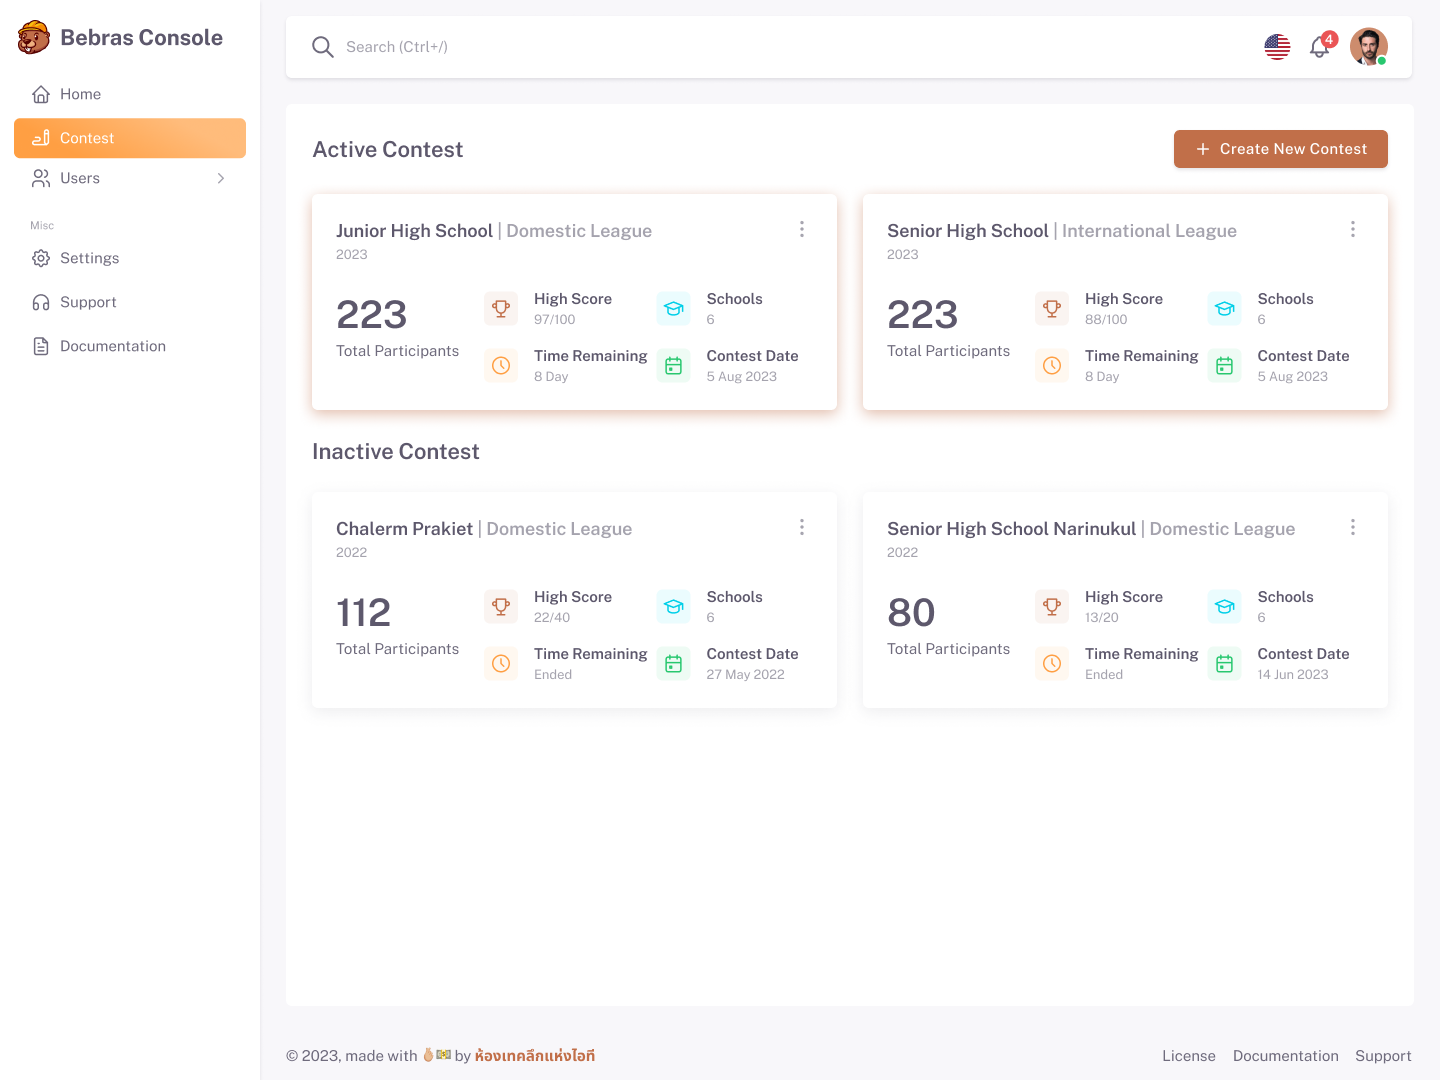
\includegraphics[width=100mm,scale=1.0]{images/admin-contest-dashboard.png}
    \caption{หน้าแสดงสถิติและประเภทการแข่งขันสำหรับผู้ดูแลระบบ}
    \label{fig:admin-contest-dashboard}
\end{figure}

การแสดงสถิติกรณีผู้ใช้คือผู้ประสานงาน (Coordinator) ผู้ใช้สามารถเห็นหน้าจอดังกล่าวซึ่งจะแสดงคะแนนต่าง ๆ ของการแข่งขันครั้งก่อนและการแข่งขันในครั้งปัจจุบัน ดังแสดงในรูปที่ \ref{fig:teacher-contest-dashboard}

\begin{figure}[H]
    \centering
    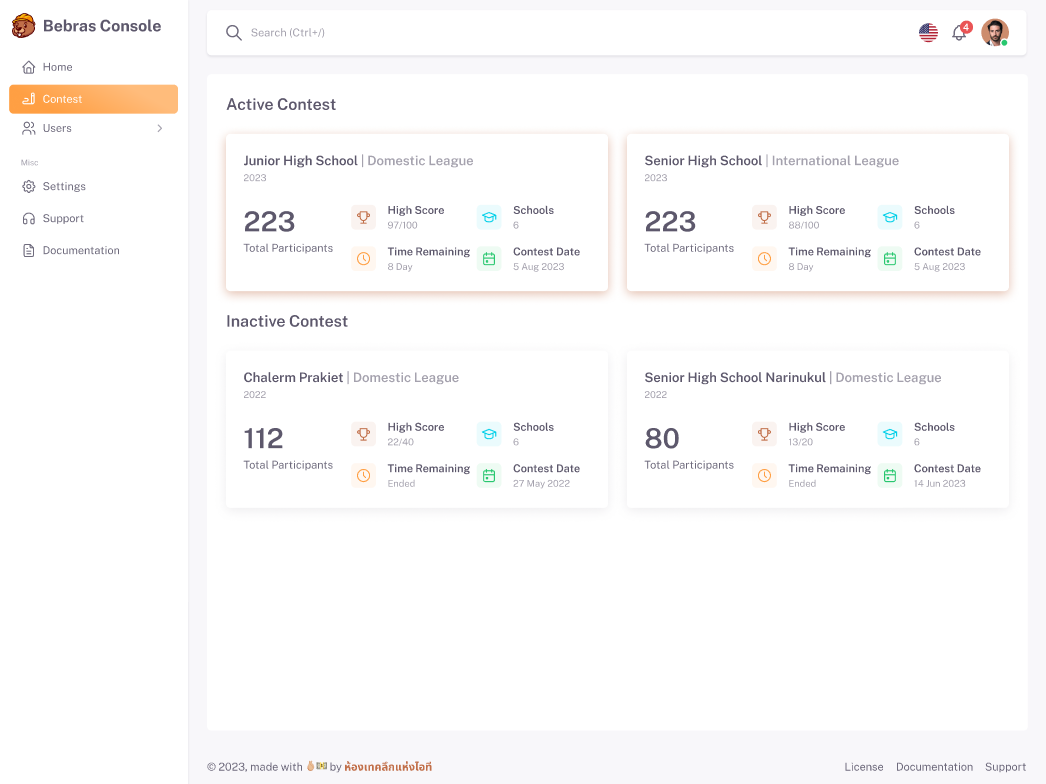
\includegraphics[width=100mm,scale=1.0]{images/teacher-contest-dashboard.png}
    \caption{หน้าแสดงสถิติและประเภทการแข่งขันสำหรับผู้ประสานงาน}
    \label{fig:teacher-contest-dashboard}
\end{figure}

\subsection{หน้าแสดงสถิติของนักเรียนในแต่ละการแข่งขัน}

การแสดงสถิติกรณีผู้ใช้คือผู้ดูแลระบบ (Admin) ผู้ใช้สามารถเห็นผลคะแนนการเข้าแข่งขันของนักเรียนแต่ละคนได้ ดังแสดงในรูปที่ \ref{fig:admin-contest-stats}

\begin{figure}[H]
    \centering
    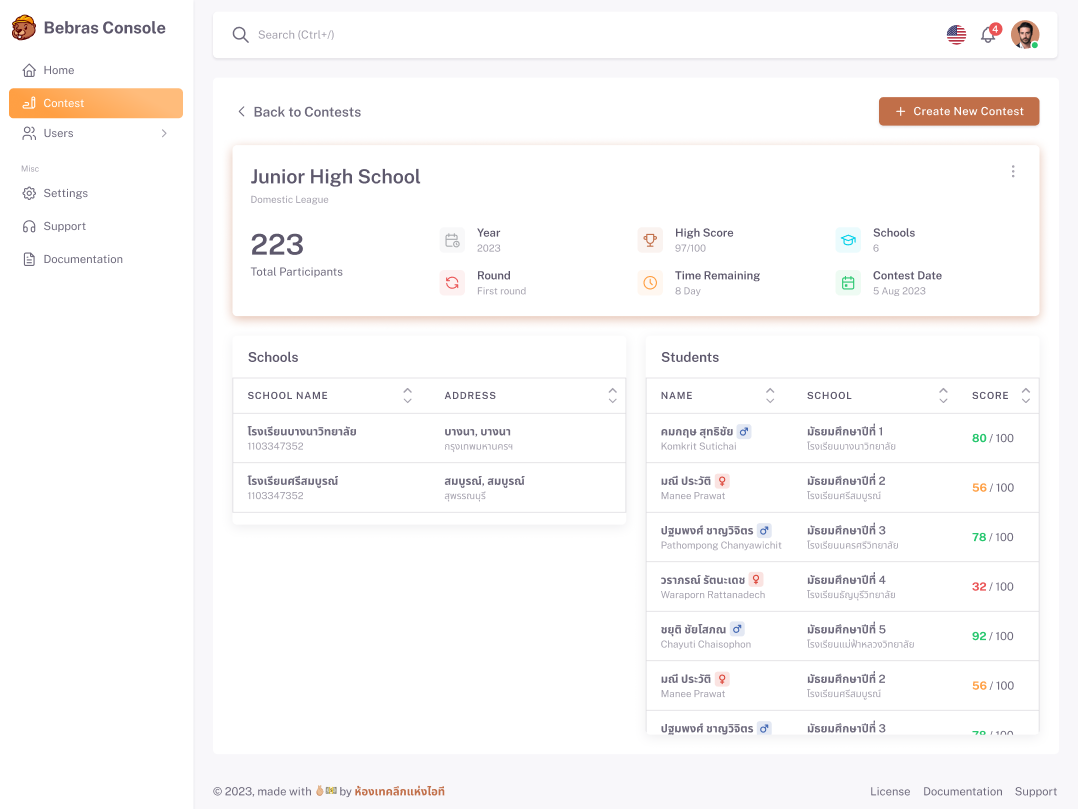
\includegraphics[width=100mm,scale=1.0]{images/admin-contest-stats.png}
    \caption{หน้าแสดงสถิติของนักเรียนในแต่ละการแข่งขันสำหรับผู้ดูแลระบบ}
    \label{fig:admin-contest-stats}
\end{figure}

การแสดงสถิติกรณีผู้ใช้คือผู้ประสานงาน (Coordinator) ผู้ใช้สามารถเห็นผลคะแนนการเข้าแข่งขันของนักเรียนแต่ละคนได้ ดังแสดงในรูปที่ \ref{fig:teacher-contest-stats}

\begin{figure}[H]
    \centering
    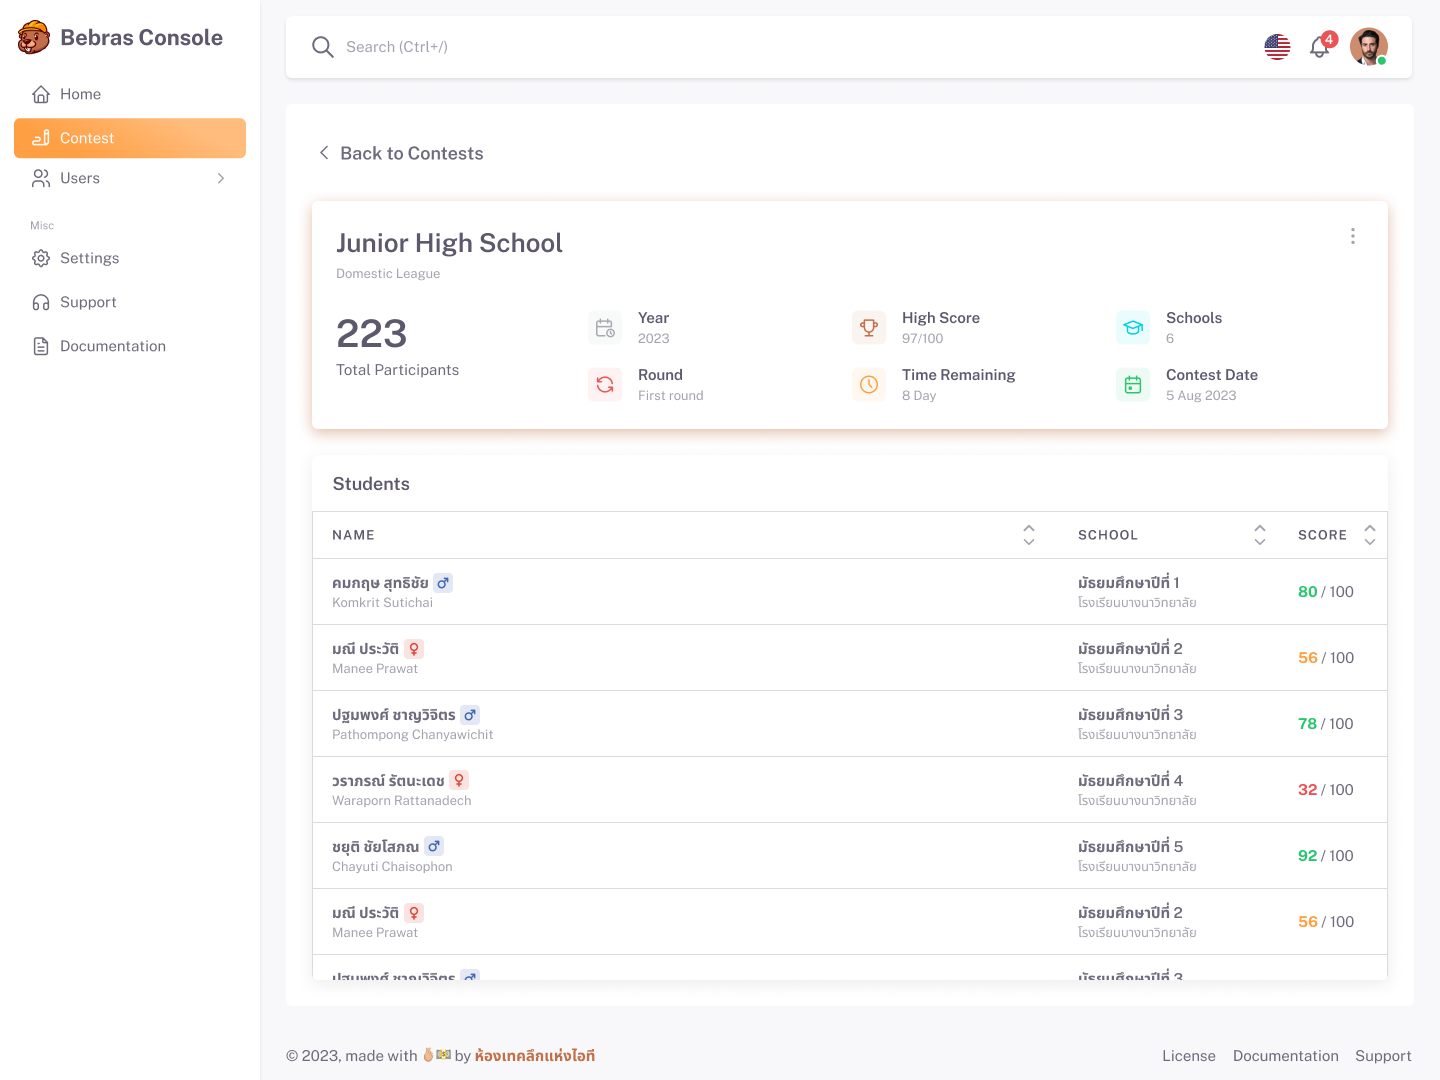
\includegraphics[width=100mm,scale=1.0]{images/teacher-contest-stats.png}
    \caption{หน้าแสดงสถิติของนักเรียนในแต่ละการแข่งขันสำหรับผู้ประสานงาน}
    \label{fig:teacher-contest-stats}
\end{figure}

\subsection{หน้าแสดงรายชื่อนักเรียน}

เมื่อเข้าสู่หน้า Student ระบบจะแสดงรายชื่อนักเรียนทั้งหมดที่มีอยู่ในระบบ โดยจะแสดงข้อมูลดังรูปที่ \ref{fig:dashboard-student}

\begin{figure}[H]
    \centering
    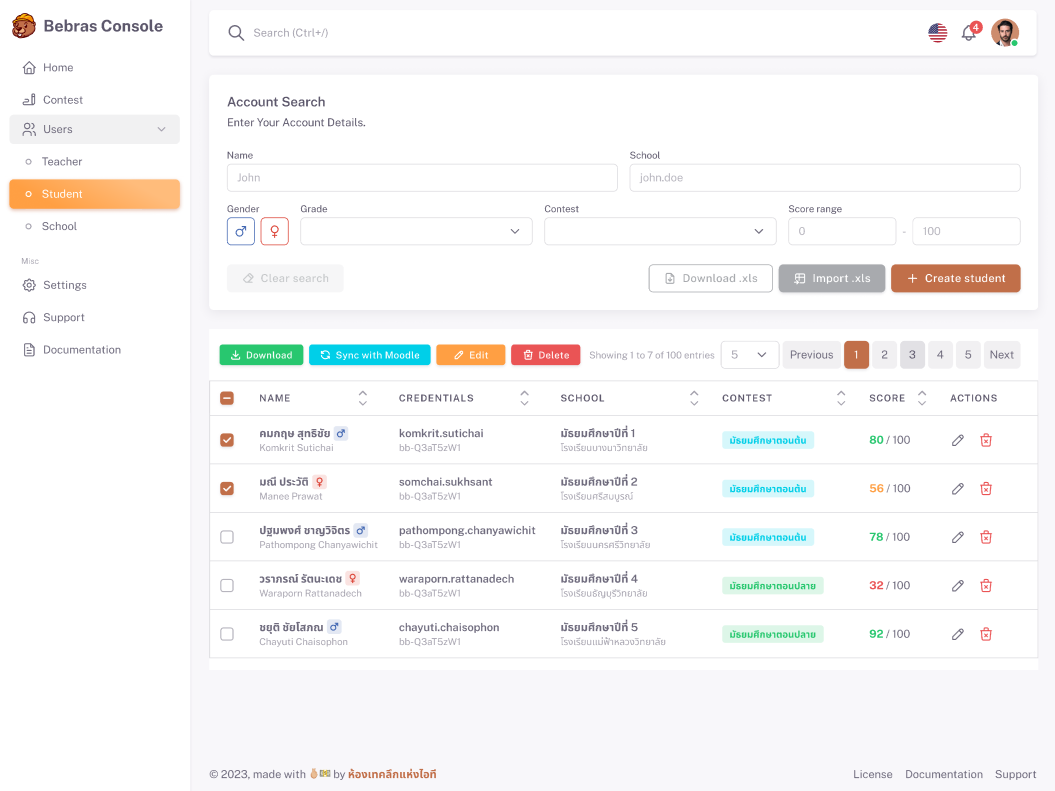
\includegraphics[width=100mm,scale=1.0]{images/student-dashboard.png}
    \caption{หน้าแสดงรายชื่อนักเรียน}
    \label{fig:dashboard-student}
\end{figure}

\subsection{หน้าเพิ่มรายชื่อนักเรียน}

ผู้ดูแลระบบ (Admin) หรือผู้ประสานงาน (Coordinator) สามารถเพิ่มข้อมูลของนักเรียน (Student) ได้ในหน้านี้โดยการคลิกที่คำว่า "Create student" เพื่อเพิ่มข้อมูลของนักเรียนลงในระบบได้ ดังแสดงในรูปที่ \ref{fig:dashboard-student} หลังจากคลิกที่ปุ่ม "Create Student" ระบบจะแสดงหน้าต่างให้กรอกข้อมูลของนักเรียน ดังแสดงในรูปที่ \ref{fig:create-student-dialog}

\begin{figure}[H]
    \centering
    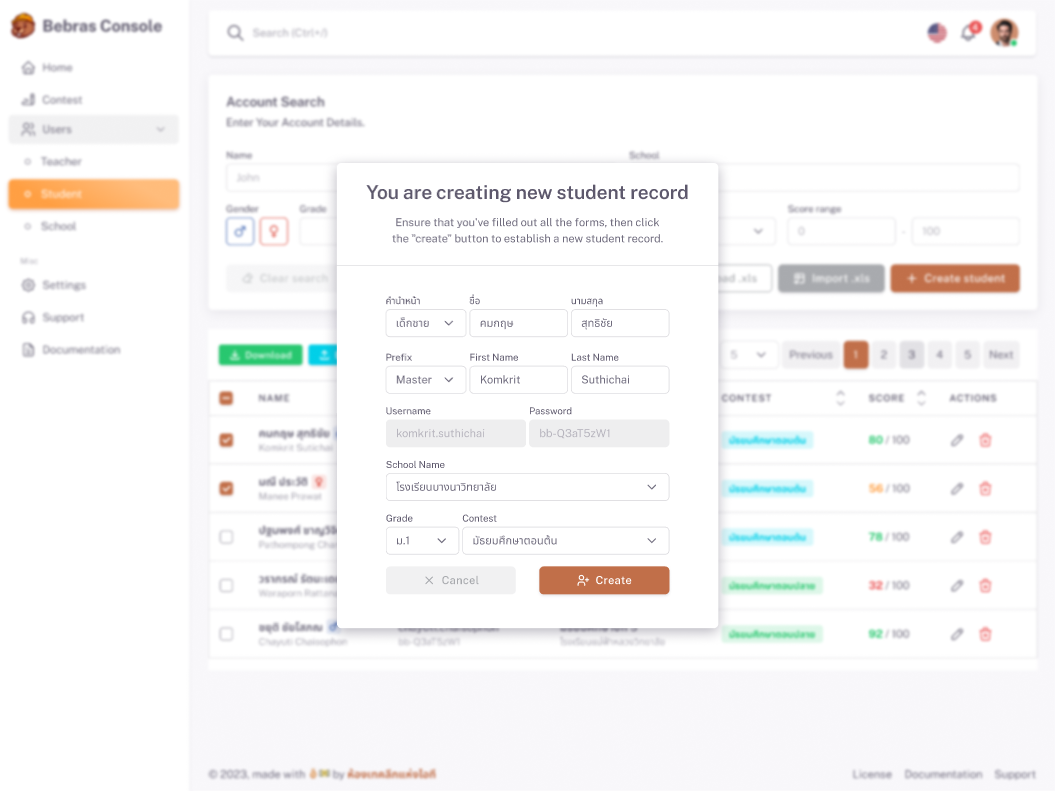
\includegraphics[width=100mm,scale=1.0]{images/create-student.png}
    \caption{หน้าเพิ่มรายชื่อนักเรียน}
    \label{fig:create-student-dialog}
\end{figure}

\subsection{หน้าลบรายชื่อนักเรียน}

ผู้ดูแลระบบ (Admin) หรือผู้ประสานงาน (Coordinator) สามารถลบข้อมูลของนักเรียน (Student) ได้ในหน้านี้โดยการคลิกที่ปุ่มถังขยะในแถวของนักเรียนที่ต้องการลบ ดังแสดงในรูปที่ \ref{fig:dashboard-student} หลังจากนั้นจะมีป๊อปอัพเพื่อให้ผู้ใช้ยืนยันก่อนทำการลบ ดังแสดงในรูปที่ \ref{fig:remove-student}

\begin{figure}[H]
    \centering
    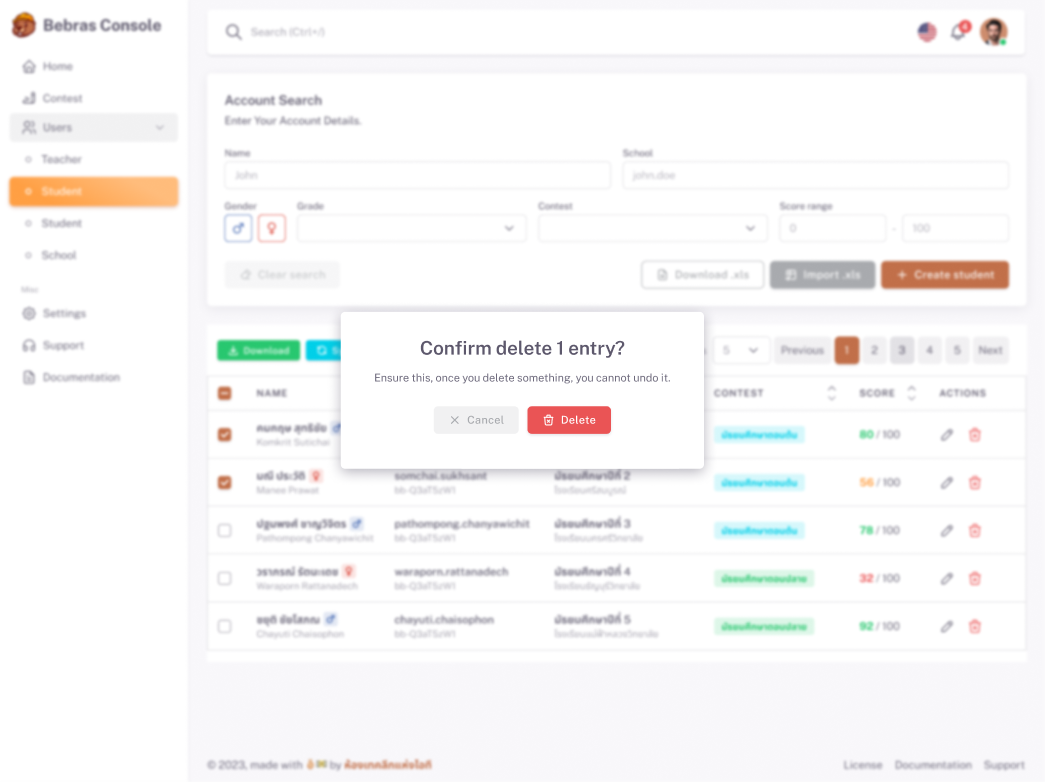
\includegraphics[width=100mm,scale=1.0]{images/remove-student.png}
    \caption{หน้าลบรายชื่อนักเรียน}
    \label{fig:remove-student}
\end{figure}